\RequirePackage[l2tabu, orthodox]{nag}
\RequirePackage{silence}
\WarningFilter{nag}{There is no environment ``centering'' }%nag complains because beamer titlepage uses a centering environment
\WarningFilter{nag}{1 complaints in total}
\WarningFilter{ifpdf}{Someone has redefined \pdfoutput}
\WarningFilter{fmtcount}{\ordinal already defined use \FCordinal instead}
\documentclass[english, french]{beamer}
%INSTALL

%avoids a warning
\usepackage[log-declarations=false]{xparse}
\usepackage{fontspec} %font selecting commands
\usepackage{xunicode}
%warn about missing characters
\tracinglostchars=2

%REDAC
\usepackage{booktabs}
\usepackage{calc}

\usepackage{mathtools} %load this before babel!
	\mathtoolsset{showonlyrefs,showmanualtags}

\usepackage{babel}
%suppresses the warning about frenchb not modifying the captions (“—” to “:” in “Figure 1 – Legend”).
	\frenchbsetup{AutoSpacePunctuation=false,SuppressWarning=false}

\usepackage[super]{nth}
\usepackage{listings} %typeset source code listings
	\lstset{language=XML,tabsize=2,literate={"}{{\tt"}}1,captionpos=b}
\usepackage[nolist,smaller,printonlyused]{acronym}%,smaller option produces warnings from relsize in some cases, it seems.
\usepackage[nodayofweek]{datetime}%must be loaded after the babel package
\usepackage{xspace}
\usepackage{hyperref}% option pdfusetitle must be introduced here, not in hypersetup.
%breaklinks makes links on multiple lines into different PDF links to the same target.
%colorlinks (false): Colors the text of links and anchors. The colors chosen depend on the the type of link. In spite of colored boxes, the colored text remains when printing.
%linkcolor=black: this leaves other links in colors, e.g. refs in green, don't print well.
%pdfborder (0 0 1, set to 0 0 0 if colorlinks): width of PDF link border
%hidelinks
\hypersetup{breaklinks,bookmarksopen,colorlinks=true,urlcolor=blue,linkcolor=,hyperfigures=true}
% hyperref doc says: Package bookmark replaces hyperref’s bookmark organization by a new algorithm (...) Therefore I recommend using this package.
\usepackage{bookmark}

% center floats by default, but do not use with float
% \usepackage{floatrow}
% \makeatletter
% \g@addto@macro\@floatboxreset\centering
% \makeatother
\usepackage{ragged2e} %new com­mands \Cen­ter­ing, \RaggedLeft, and \RaggedRight and new en­vi­ron­ments Cen­ter, FlushLeft, and FlushRight, which set ragged text and are eas­ily con­fig­urable to al­low hy­phen­ation (the cor­re­spond­ing com­mands in LaTeX, all of whose names are lower-case, pre­vent hy­phen­ation al­to­gether). 
\usepackage{siunitx} %[expproduct=tighttimes, decimalsymbol=comma]
\sisetup{detect-all}% to detect e.g. when in math mode (use a math font)
\usepackage{braket} %for \Set
\usepackage{natbib}

\usepackage{amsmath,amsthm}
% \usepackage{amsfonts} %not required?
% \usepackage{dsfont} %for what?
%unicode-math overwrites the following commands from the mathtools package: \dblcolon, \coloneqq, \Coloneqq, \eqqcolon. Using the other colon-like commands from mathtools will lead to inconsistencies. Plus, Using \overbracket and \underbracke from mathtools package. Use \Uoverbracket and \Uunderbracke for original unicode-math definition.
%use exclusively \mathbf and choose math bold style below.
\usepackage[warnings-off={mathtools-colon, mathtools-overbracket}, bold-style=ISO]{unicode-math}

\defaultfontfeatures{
	Fractions=On,
	Mapping=tex-text% to turn "--" into dashes, useful for bibtex%%
}
\defaultfontfeatures[\rmfamily, \sffamily]{
	Fractions=On,
	Mapping=% to leave " alone (disable the default mapping tex-text; requires loading the font afterwards?)
}
\newfontfamily\xitsfamily{XITS}
\newfontfamily\texgyretermesfamily{TeX Gyre Termes}
\newfontfamily\texgyreherosfamily{TeX Gyre Heros}
\newfontfamily\lmfamily{Latin Modern Roman}
\setmainfont{Latin Modern Roman}
\setsansfont{Latin Modern Sans}
\setmonofont{Latin Modern Mono}
\defaultfontfeatures{}%disable default font features to avoid warnings with math fonts.
\setmathfont{XITS Math}
\setmathfont[range={\mathcal,\mathbfcal},StylisticSet=1]{XITS Math}

\usepackage{cleveref}% cleveref should go "laster" than hyperref
%GRAPHICS
\usepackage{pgf}
\usepackage{pgfplots}
	\usetikzlibrary{matrix,fit,plotmarks,calc,trees,shapes.geometric,positioning,plothandlers}
\pgfplotsset{compat=1.11}
\usepackage{graphicx}

\graphicspath{{graphics/},{graphics-dm/}}
\DeclareGraphicsExtensions{.pdf}

%HACKING
\usepackage{printlen}
\uselengthunit{mm}
% 	\newlength{\templ}% or LenTemp?
% 	\setlength{\templ}{6 pt}
% 	\printlength{\templ}
\usepackage{etoolbox} %for addtocmd command
\usepackage{scrhack}% load at end. Corrects a bug in float package, which is outdated but might be used by other packages
\usepackage{xltxtra} %somebody said that this is loaded by fontspec, but does not seem correct: if not loaded explicitly, does not appear in the log and \showhyphens is not corrected.

%Beamer-specific
%ADD
\usepackage{appendixnumberbeamer}
%\setbeamersize{text margin left=0.1cm, text margin right=0.1cm} 
\setbeamertemplate{navigation symbols}{}
\usetheme{BrusselsBelgium}
\usefonttheme{professionalfonts}


\newcommand{\R}{ℝ}
\newcommand{\N}{ℕ}
\newcommand{\Z}{ℤ}
\newcommand{\card}[1]{\lvert{#1}\rvert}
\newcommand{\powerset}[1]{\mathscr{P}(#1)}%\mathscr rather than \mathcal: scr is rounder than cal (at least in XITS Math).
\newcommand{\suchthat}{\;\ifnum\currentgrouptype=16 \middle\fi|\;}
%\newcommand{\Rplus}{\reels^+\xspace}

\AtBeginDocument{%
	\renewcommand{\epsilon}{\varepsilon}
% we want straight form of \phi for mathematics, as recommended in UTR #25: Unicode support for mathematics.
%	\renewcommand{\phi}{\varphi}
}

% with amssymb, but I don’t want to use amssymb just for that.
% \newcommand{\restr}[2]{{#1}_{\restriction #2}}
%\newcommand{\restr}[2]{{#1\upharpoonright}_{#2}}
\newcommand{\restr}[2]{{#1|}_{#2}}%sometimes typed out incorrectly within \set.
%\newcommand{\restr}[2]{{#1}_{\vert #2}}%\vert errors when used within \Set and is typed out incorrectly within \set.
\DeclareMathOperator*{\argmax}{arg\,max}
\DeclareMathOperator*{\argmin}{arg\,min}


%ARG TH
\newcommand{\AF}{\mathcal{AF}}
\newcommand{\labelling}{\mathcal{L}}
\newcommand{\labin}{\textbf{in}\xspace}
\newcommand{\labout}{\textbf{out}}
\newcommand{\labund}{\textbf{undec}\xspace}
\newcommand{\nonemptyor}[2]{\ifthenelse{\equal{#1}{}}{#2}{#1}}
\newcommand{\gextlab}[2][]{
	\labelling{\mathcal{GE}}_{(#2, \nonemptyor{#1}{\ibeatsr{#2}})}
}
\newcommand{\allargs}{A^*}
\newcommand{\args}{A}
\newcommand{\ar}{a}

%MCDA+Arg
\newcommand{\dm}{d}
\newcommand{\ileadsto}{\leadsto}
\newcommand{\mleadsto}[1][\eta]{\leadsto_{#1}}
\newcommand{\ibeats}{\vartriangleright}
\newcommand{\mbeats}[1][\eta]{\vartriangleright_{#1}}


%MISC
\newcommand{\lequiv}{\Vvdash}
\newcommand{\weightst}{W^{\,t}}

%MCDA classical
\newcommand{\crits}{\mathcal{J}}
\newcommand{\altspace}{\mathbb{A}}
\newcommand{\alts}{A}

%Sorting
\newcommand{\cats}{\mathcal{C}}
\newcommand{\catssubsets}{2^\cats}
\newcommand{\catgg}{\vartriangleright}
\newcommand{\catll}{\vartriangleleft}
\newcommand{\catleq}{\trianglelefteq}
\newcommand{\catgeq}{\trianglerighteq}
\newcommand{\alttoc}[2][x]{(#1 \xrightarrow{} #2)}
\newcommand{\alttocat}[3]{(#2 \xrightarrow{#1} #3)}
\newcommand{\alttoI}{(x \xrightarrow{} \left[\underline{C_x}, \overline{C_x}\right])}
\newcommand{\alttocatdm}[3][t]{\left(#2 \thinspace \raisebox{-3pt}{$\xrightarrow{#1}$}\thinspace #3\right)}
\newcommand{\alttocatatleast}[2]{\left(#1 \thinspace \raisebox{-3pt}{$\xrightarrow[]{≥}$}\thinspace #2\right)}
\newcommand{\alttocatatmost}[2]{\left(#1 \thinspace \raisebox{-3pt}{$\xrightarrow[]{≤}$}\thinspace #2\right)}

\newcommand{\source}{\scriptsize}
\newcommand{\commentOC}[1]{{\selectlanguage{french}{\todo{OC : #1}}}}
%Or: \todo[color=green!40]

%this probably requires outdated float package, see doc KomaScript for an alternative.
% \newfloat{program}{t}{lop}
% \floatname{program}{PM}

%\crefname{axiom}{axiom}{axioms}%might be needed for workaround bug in cref when defining new theorems?

%\ifdefined\theorem\else
%\newtheorem{theorem}{\iflanguage{english}{Theorem}{Théorème}}
%\fi

%which line breaks are chosen: accept worse lines, therefore reducing risk of overfull lines. Default = 200
\tolerance=2000
%accept overfull hbox up to...
\hfuzz=2cm
%reduces verbosity about the bad line breaks
\hbadness 5000
%sloppy sets tolerance to 9999
\apptocmd{\sloppy}{\hbadness 10000\relax}{}{}

% WRITING
%\newcommand{\ie}{i.e.\@\xspace}%to try
%\newcommand{\eg}{e.g.\@\xspace}
%\newcommand{\etal}{et al.\@\xspace}
\newcommand{\ie}{i.e.\ }
\newcommand{\eg}{e.g.\ }
\newcommand{\mkkOK}{\checkmark}%\color{green}{\checkmark}
\newcommand{\mkkREQ}{\ding{53}}%requires pifont?%\color{green}{\checkmark}
\newcommand{\mkkNO}{}%\text{\color{red}{\textsf{X}}}

\makeatletter
\newcommand{\boldor}[2]{%
	\ifnum\strcmp{\f@series}{bx}=\z@
		#1%
	\else
		#2%
	\fi
}
\newcommand{\textstyleElProm}[1]{\boldor{\MakeUppercase{#1}}{\textsc{#1}}}
\makeatother
\newcommand{\electre}{\textstyleElProm{Électre}\xspace}
\newcommand{\electreIv}{\textstyleElProm{Électre Iv}\xspace}
\newcommand{\electreIV}{\textstyleElProm{Électre IV}\xspace}
\newcommand{\electreIII}{\textstyleElProm{Électre III}\xspace}
\newcommand{\electreTRI}{\textstyleElProm{Électre Tri}\xspace}
% \newcommand{\utadis}{\texorpdfstring{\textstyleElProm{utadis}\xspace}{UTADIS}}
% \newcommand{\utadisI}{\texorpdfstring{\textstyleElProm{utadis i}\xspace}{UTADIS I}}

%TODO
% \newcommand{\textstyleElProm}[1]{{\rmfamily\textsc{#1}}} 


\newlength{\GraphsNodeSep}
\setlength{\GraphsNodeSep}{7mm}

% MCDA Drawing Sorting
\newlength{\MCDSCatHeight}
\setlength{\MCDSCatHeight}{6mm}
\newlength{\MCDSAltHeight}
\setlength{\MCDSAltHeight}{4mm}
%separation between two vertical alts
\newlength{\MCDSAltSep}
\setlength{\MCDSAltSep}{2mm}
\newlength{\MCDSCatWidth}
\setlength{\MCDSCatWidth}{3cm}
\newlength{\MCDSEvalRowHeight}
\setlength{\MCDSEvalRowHeight}{6mm}
\newlength{\MCDSAltsToCatsSep}
\setlength{\MCDSAltsToCatsSep}{1.5cm}
\newcounter{MCDSNbAlts}
\newcounter{MCDSNbCats}
\newlength{\MCDSArrowDownOffset}
\setlength{\MCDSArrowDownOffset}{0mm}

\tikzset{/Graphs/dot/.style={
	shape=circle, fill=black, inner sep=0, minimum size=1mm
}}
\tikzset{/MC/D/S/alt/.style={
	shape=rectangle, draw=black, inner sep=0, minimum height=\MCDSAltHeight, minimum width=2.5cm, anchor=north east
}}
\tikzset{MC/D/S/pref/.style={
	shape=ellipse, draw=gray, thick
}}
\tikzset{/MC/D/S/cat/.style={
	shape=rectangle, draw=black, inner sep=0, minimum height=\MCDSCatHeight, minimum width=\MCDSCatWidth, anchor=north west
}}
\tikzset{/MC/D/S/evals matrix/.style={
	matrix, row sep=-\pgflinewidth, column sep=-\pgflinewidth, nodes={shape=rectangle, draw=black, inner sep=0mm, text depth=0.5ex, text height=1em, minimum height=\MCDSEvalRowHeight, minimum width=12mm}, nodes in empty cells, matrix of nodes, inner sep=0mm, outer sep=0mm, row 1/.style={nodes={draw=none, minimum height=0em, text height=, inner ysep=1mm}}
}}

% Beliefs
\tikzset{/Beliefs/D/S/attacker/.style={
	shape=rectangle, draw, minimum size=8mm
}}
\tikzset{/Beliefs/D/S/supporter/.style={
	shape=circle, draw
}}

\newcommand{\tikzmark}[1]{%
	\tikz[overlay, remember picture, baseline=(#1.base)] \node (#1) {};%
}


\begin{acronym}
\acro{AMCD}{Aide Multicritère à la Décision}
\acro{ASA}{Argument Strength Assessment}
\acro{DA}{Decision Analysis}
\acro{DM}{Decision Maker}
\acro{DPr}{Deliberated Preferences}
\acro{DRSA}{Dominance-based Rough Set Approach}
\acro{DSS}{Decision Support Systems}
\acrodefplural{DSS}{Decision Support Systems}
% \newacroplural{DSS}[DSSes]{Decision Support Systems}
\acro{EJOR}{European Journal of Operational Research}
\acro{LNCS}{Lecture Notes in Computer Science}
\acro{MCDA}{Multicriteria Decision Aid}
\acro{MIP}{Mixed Integer Program}
\acro{NCSM}{Non Compensatory Sorting Model}
\acro{PL}{Programme Linéaire}
\acro{PLNE}{Programme Linéaire en Nombres Entiers}
\acro{PM}{Programme Mathématique}
\acro{MP}{Mathematical Program}
\acro{MIP}{Mixed Integer Program}
% \newacroplural{PM}{Programmes Mathématiques}
%acrodefplural since version 1.35, my debian has \ProvidesPackage{acronym}[2009/01/25, v1.34, Support for acronyms (Tobias Oetiker)]
\acrodefplural{PM}{Programmes Mathématiques}
\acro{PMML}{Predictive Model Markup Language}
\acro{RESS}{Reliability Engineering \& System Safety}
\acro{SMAA}{Stochastic Multicriteria Acceptability Analysis}
\acro{URPDM}{Uncertainty and Robustness in Planning and Decision Making}
\acro{XML}{Extensible Markup Language}
\end{acronym}


\title{Conception d’applications internet}
\subtitle{Introduction}
\subject{Java EE}
\keywords{EJB, deployment, modules, servlet}
\author{Olivier Cailloux}
\institute[LAMSADE]{LAMSADE, Université Paris-Dauphine}
\date{\formatdate{12}{11}{2015}}

\begin{document}
\bibliographystyle{apalike}

\begin{frame}[plain]
	\tikz[remember picture,overlay]{
		\path (current page.south west) node[anchor=south west, inner sep=0] {
			
\includegraphics[height=1cm]{LAMSADE95.jpg}
		};
		\path (current page.south) ++ (0, 1mm) node[anchor=south, inner sep=0] {
			
\includegraphics[height=9mm]{Dauphine.jpg}
		};
		\path (current page.south east) node[anchor=south east, inner sep=0] {
			
\includegraphics[height=1cm]{PSL.png}
		};
	}
   \titlepage
\end{frame}
\addtocounter{framenumber}{-1}

\section{Présentations}
\subsection{L’enseignant}
\begin{frame}
	\frametitle{L’enseignant}
	\begin{itemize}
		\item Olivier Cailloux
		\item \href{mailto:olivier.cailloux@dauphine.fr}{olivier.cailloux@dauphine.fr}
		\item Coordonnées : cf. \href{https://www.ent.dauphine.fr/Annuaire/index.php?param0=fiche&param1=ocailloux}{annuaire} de Dauphine
	\end{itemize}
\end{frame}

\subsection{Java}
\begin{frame}[fragile]
	\frametitle{Le terme Java}
	
	Terme \emph{Java} adopté en 1995 (“as an example of yet another name that would never work”) \source{(source: \href{http://www.javaworld.com/article/2077265/core-java/so-why-did-they-decide-to-call-it-java-.html}{Java World})}
	\hfill
	\vfill
	\begin{minipage}[b]{3cm}
		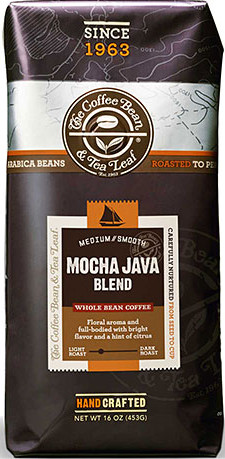
\includegraphics[height=5.5cm]{Java_beans.jpg}
	\end{minipage}%
	\begin{minipage}[b]{(\columnwidth - 3cm)}
		\centering{
\includegraphics[height=9mm]{java-icon.png}}
		\pause
		\href{https://en.wikipedia.org/wiki/Java}{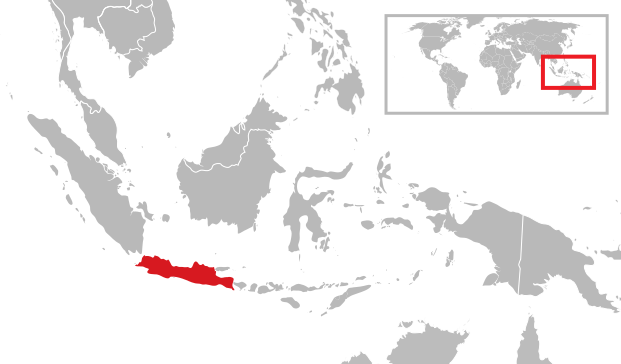
\includegraphics[width=\columnwidth]{Java_Locator.svg.png}}
%		\mbox{} \raggedleft \source{Gunawan Kartapranata - \href{https://en.wikipedia.org/wiki/Java}{wikipedia}}
	\end{minipage}
\end{frame}

\begin{frame}
	\frametitle{A jar full of Java beans, please}
	\begin{itemize}
		\item JAR File : introduits à la version 1.1. Une collection de fichiers \texttt{.class}.
		\item Java Bean (aussi version 1.1). (\href{http://www.oracle.com/technetwork/java/javase/documentation/spec-136004.html}{specs}) : un composant logiciel pour assemblage (par exemple, un bouton AWT, une feuille de calcul à placer dans un document).
	\end{itemize}
	\centering{
		\href{http://houseofjava.ca/}{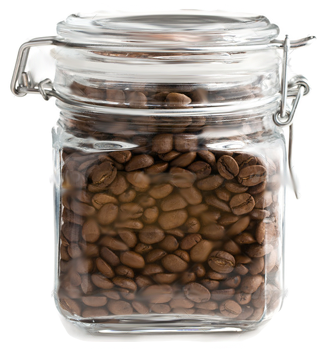
\includegraphics[height=3cm]{bean-jar.png}}
	}
	\begin{block}{Fun fact}
		Voyons le nombre magique des fichiers \texttt{.class}…
	\end{block}
\end{frame}

\subsection{Java EE}
\begin{frame}
	\frametitle{Java EE}
	\begin{itemize}
		\item Java EE ? \pause Java Platform, Enterprise Edition \pause
		\item JCP ? \pause Java Community Process \pause
		\item API ? \pause Application Programming Interface \pause
	\end{itemize}
	\begin{block}{Java EE}
		\begin{itemize}
			\item \href{http://www.oracle.com/technetwork/java/javaee/tech/index.html}{technologies}
			\item Spécifications, dont API
			\item Implémentation de référence
			\item Version actuelle : 7
		\end{itemize}
	\end{block}
\end{frame}

\section{Objectifs pédagogiques}
\subsection{Objectifs pédagogiques}
\begin{frame}
	\frametitle{Objectifs pédagogiques, 1}
	\begin{block}{Mise en œuvre des patterns}
		\begin{itemize}
		\item Mise en œuvre des patterns dans les spécifications Java EE
		\item Quand les mettre en œuvre ?
		\item Applications dans programmes propres
		\end{itemize}
	\end{block}
\end{frame}

\begin{frame}
	\frametitle{Objectifs pédagogiques, 2}
	\begin{block}{Lecture de spécifications}
		\begin{itemize}
		\item Savoir extraire l’information utile des spécifications !
		\item Standards W3C, spécifications Java EE…
		\end{itemize}
	\end{block}
\end{frame}

\begin{frame}
	\frametitle{Objectifs pédagogiques, 3}
	\begin{block}{Modélisation}
		\begin{itemize}
		\item Réponse à des besoins exprimés vaguement
		\item Appui sur les standards du web actuels
		\item Dosage du réalisme et de l’intérêt des fonctionalités
		\end{itemize}
	\end{block}
	Quels sont \emph{vos} objectifs ?
\end{frame}

\subsection{Utilité}
\begin{frame}
	\frametitle{Intérêt pratique}
	\begin{itemize}
		\item Qu’on soit programmeur, qu’on discute avec des programmeurs
		\item Rendre le travail plus difficile conceptuellement
		\item Prendre de la hauteur, éviter les tâches répétitives et se concentrer sur le conceptuel
		\item Respect et compréhension des standards (aperçu de la façon dont ils sont construits) : compétence essentielle
		\item … dans de multiples domaines
		\item Importance des patterns dans de multiples domaines
		\item Technologie en vogue
	\end{itemize}
\end{frame}

\section{Moyens}
\subsection{Théorie}
\begin{frame}
	\frametitle{Par cours}
	À l’issue de chaque (?) cours :
	\begin{itemize}
		\item compréhension des bases théoriques d’une technologie (patterns invoqués, liens avec autres technologies)
		\item capacité de réponse à l’aide de la technologie vue à (au moins) un besoin simple
	\end{itemize}
\end{frame}

\subsection{Projet}
\begin{frame}
	\frametitle{Projet}
	\begin{itemize}
		\item Réponse à un besoin \emph{réel}
		\item Par groupe
		\item Pair programming encouragé
		\item Rapport final
		\item Recommandé : code en anglais
	\end{itemize}
\end{frame}

\subsection{Forum}
\begin{frame}
	\frametitle{Forum}
	\begin{itemize}
		\item Sur My Course
		\item Marquer les posts utiles !
	\end{itemize}
\end{frame}

\subsection{Évaluation}
\begin{frame}
	\frametitle{Évaluation}
	Résultat : 0,7 × note projet finale + 0,3 × note concept.
	\begin{block}{Projet}
		\begin{itemize}
			\item Évaluation projet final pondérée par code individuel
			\item Indiquez (qui commet et) qui est support
			\item Le rapport peut servir à expliquer des déséquilibres
			\item Un faible pilotage ne sera pas compensé par un grand support
			\item Si vous avez testé le pair programming : mieux
		\end{itemize}
	\end{block}
	\begin{block}{Concept}
		Résumé, tuto, note critique, document explicatif, vidéo, correction de wikipedia, réponses sur stackexchange, sur le forum, code…
	\end{block}
	Vote pour le meilleur pédagogue et pour le meilleur projet
\end{frame}

\subsection{Prérequis}
\begin{frame}
	\frametitle{Prérequis}
	Programmation Java théorique et appliquée ; ingénieurie logicielle théorique
	\begin{itemize}
		\item Exceptions
		\item Héritage
		\item Concept d’API
		\item Programmation par contrat
		\item XML
		\item Maven
		\item Git
	\end{itemize}
\end{frame}

\section{Java EE}
\subsection{Processus}
\begin{frame}
	\frametitle{Java EE : Processus}
	\begin{itemize}
		\item Java EE fortement appuyée sur standards ouverts
		\item Standards du W3C / IETF ?\pause{} \href{http://www.w3.org/Protocols/}{HTTP}, \href{http://www.w3.org/html/}{HTML}, \href{http://www.w3.org/XML/}{XML}, \href{http://www.w3.org/TR/wsdl}{WSDL}, …\pause
		\item JCP : implication de \og{}la communauté\fg{} pour standards Java
		\item Tentions entre standard ouvert et contrôle ! (2010, Apache \href{https://blogs.apache.org/foundation/entry/the_asf_resigns_from_the}{quitte} le comité JCP ; Doug Lea \href{http://gee.cs.oswego.edu/dl/html/jcp22oct10.html}{également}, en faveur de OpenJDK…)
	\end{itemize}
\end{frame}

\subsection{Conteneurs}
\begin{frame}
	\frametitle{Conteneurs}
	\begin{itemize}
		\item Un produit conforme Java EE fournit trois \emph{conteneurs}
		\begin{itemize}
			\item Conteneur EJB
			\item Conteneur web
			\item Conteneur application client
		\end{itemize}
		\item Contenant des \emph{composants} (du type adéquat)
		\item Chacun fournit des services pour le développeur
		\item Fournit l’accès aux API (différents conteneurs, différentes API)
%		\item Différents conteneurs donnent accès à différentes API (ex : pas Web Socket dans EJB conteneur)
	\end{itemize}
%	\begin{block}{Conteneurs}
%	\end{block}
	\href{https://docs.oracle.com/javaee/7/tutorial/overview007.htm}{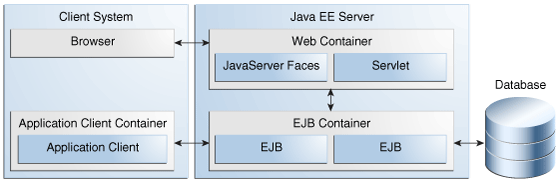
\includegraphics[width=\columnwidth]{containers.png}}
\end{frame}

\subsection{Composants}
\begin{frame}
	\frametitle{Composants}
	\begin{itemize}
		\item \emph{Composant} : une unité logicielle assemblée dans une application Java EE avec ses classes et fichiers liés et communiquant avec d’autres composants.
		\item Code Java compilé normalement
		\item Assemblé dans une application Java EE : peut utiliser les services ; doit se conformer aux spécifications
		\item Exécution gérée par le conteneur (pas de \texttt{main}, par exemple)
	\end{itemize}
\end{frame}

\begin{frame}
	\frametitle{Composant EJB}
	\begin{block}{EJB}
		\begin{itemize}
			\item \emph{Enterprise} Java Bean
			\item Composant \og{}business\fg{}, sur le serveur
			\item Service pouvant être appelé localement ou à distance
			\item Deux types : session bean, message-driven bean
		\end{itemize}
	\end{block}
	\begin{itemize}
		\item Le conteneur rend l’EJB accessible de l’extérieur
		\item Permet le Remote Method Invocation, sorte de RPC
		\item Le conteneur instancie, facilite la sérialisation, …
	\end{itemize}
\end{frame}

\begin{frame}
	\frametitle{Composant Web}
	\begin{itemize}
		\item Java Servlet
		\item JavaServer Faces
	\end{itemize}
\end{frame}

\subsection{Couches}
\begin{frame}
	\frametitle{Couches (\og{}tier\fg{})}
	\begin{minipage}{\columnwidth*\real{0.6}}
		\href{https://docs.oracle.com/javaee/7/tutorial/overview003.htm}{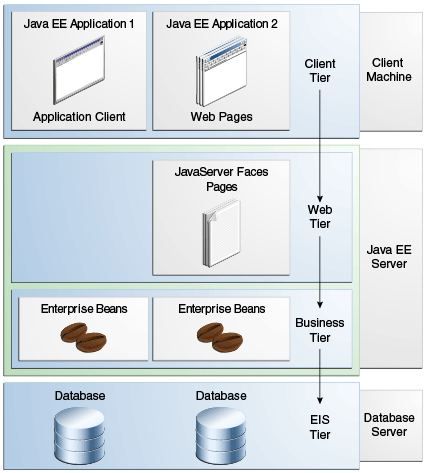
\includegraphics[width=\columnwidth]{tiers.png}}
	\end{minipage}%
	\begin{minipage}{\columnwidth*\real{0.4}}
		\begin{itemize}
			\item Ajout d’une couche multithread entre le client et le serveur classique
			\item Souvent : presentation, logic, data tier
			\item Couche web : peut être également appelé un client web (pourquoi ?).
		\end{itemize}
	\end{minipage}
\end{frame}

\subsection{Exemples d’applications}
\begin{frame}
	\frametitle{Deux applications Java EE}
	\begin{block}{BDD $⇔$ EJB $⇔$ client}
		\begin{itemize}
			\item entreprise A : niveau de stock calculable d’après BDD
			\item EJB : requête pour obtenir le niveau de stock
			\item composant client (fournisseur de A) : contacte l’EJB
		\end{itemize}		
	\end{block}
	
	\begin{block}{BDD $⇔$ EJB $⇔$ Servlet}
		\begin{itemize}
			\item entreprise A : niveau de stock calculable d’après BDD
			\item EJB : requête pour obtenir le niveau de stock
			\item Web : servlet répondant à HTTP GET (client léger)
			\item Et puis ? Quel client final ?
		\end{itemize}		
	\end{block}
	
	Options pour client non-java ?
\end{frame}

\subsection{Assemblage et déploiement}
\begin{frame}
	\frametitle{Modules}
	\begin{itemize}
		\item \emph{Module} Java EE : fichier archive compressé
		\item Ensemble de composants pour un même conteneur {\tiny (typiquement)}
		\item Éventuellement : un descripteur de déploiement (\texttt{.xml}) pour ce type de conteneur (standard Java EE ou par produit)
		\item Éventuellement :  des pages HTML statiques ; des classes utilité, …
		\item Les descripteurs surchargent les annotations
	\end{itemize}
\end{frame}

\begin{frame}
	\frametitle{Module Web}
	\begin{block}{Module Web}
		\begin{itemize}
			\item Fichier \texttt{.war}
			\item Fichiers \texttt{.class} servlets et autres dans WEB-INF/lib ou WEB-INF/classes
			\item Fichiers web statiques (.html, images, …) dans root
			\item \texttt{WEB-INF/web.xml} : descripteur pour conteneur Web (JNDI)
			\item \texttt{META-INF/glassfish-web.xml} : descripteur pour glassfish
			\item \texttt{META-INF/MANIFEST.MF}
		\end{itemize}
	\end{block}
%	\begin{block}{Module EJB}
%		\begin{itemize}
%			\item Fichier \texttt{.jar}
%			\item Fichiers \texttt{.class} EJB et autres
%			\item \texttt{META-INF/ejb-jar.xml} : descripteur pour conteneur EJB (attributs de transaction, sécurité, …)
%			\item \texttt{META-INF/glassfish-ejb-jar.xml} : descripteur pour glassfish
%			\item \texttt{META-INF/MANIFEST.MF}
%		\end{itemize}
%	\end{block}
%	\item Application client modules (class files and, optionally, an application client deployment descriptor) : \texttt{.jar}.
%	\item (Resource adapter modules : \texttt{.rar}.)
%    , which contain all Java interfaces, classes, native libraries, and, optionally, a resource adapter deployment descriptor. Together, these implement the Connector architecture (see Java EE Connector Architecture) for a particular EIS. Resource adapter modules are packaged as JAR files with an .rar (resource adapter archive) extension.
\end{frame}

\begin{frame}
	\frametitle{Assemblage et déploiement}
	\begin{itemize}
		\item Application Java EE composée d’un ou plusieurs modules
		\item On peut déployer un module seul (\texttt{.war}, \texttt{.jar})
		\item Ou assembler les modules dans un fichier Enterprise Archive (\texttt{.ear})
		\item EAR : plusieurs modules et év. descripteur d’application (\texttt{META-INF/application.xml}, \texttt{META-INF/glassfish-application.xml})
	\end{itemize}
	\begin{block}{Déploiement}
		\begin{itemize}
			\item Procédure dépend du serveur d’application Java EE
			\item Typiquement : déplacer l’archive (\texttt{.war}, \texttt{.ear}, \texttt{.jar}) dans un répertoire du serveur
			\item Accès depuis l’environnement de développement via plug-ins
		\end{itemize}
	\end{block}
\end{frame}

\subsection{Services}
\begin{frame}
	\frametitle{Services}
	Exemples :
	\begin{itemize}
		\item Managed beans
		\item CDI
		\item RestFul
		\item JSF
		\item Bean validation
		\item JAXB, JAX-WS, JNDI (aussi dans Java SE)
	\end{itemize}
\end{frame}

\subsection{GlassFish}
\begin{frame}
	\frametitle{GlassFish Server Tools}
	\begin{itemize}
		\item Démarrer, arrêter le serveur
		\item Déployer des paquets
		\item Application : console d’administration
		\item Base de données
		\item wsimport : artéfacts JAX-WS depuis WSDL (etc.)
	\end{itemize}
	\begin{block}{À vous}
		\begin{itemize}
			\item \og{}Installez\fg{} GlassFish (copie depuis \texttt{/usr/local/glassfish-4.1/glassfish})
			\item Démarrez votre serveur (cf. \texttt{bin/}, \url{http://localhost:8080}, \url{http://localhost:4848})
			\item Désactivez l’écoute extérieure
			\item Lisez les logs
		\end{itemize}
	\end{block}
\end{frame}

\section[Un servlet]{Mon premier servlet}
\subsection{En Eclipse}
\begin{frame}
	\frametitle{Accès environnement Java EE via Eclipse}
	\begin{itemize}
		\item Accès aux bibliothèques Java EE requis
		\item En Eclipse : possible d’ajouter un environnement Java EE rudimentaire, \og{}J2EE Preview\fg{} (Preferences / Server / Runtime Environments)
		\item Quand un projet vise ce runtime, eclipse ajoute les bibliothèques en dépendances
		\item Ces bibliothèques ne seront cependant pas exportées dans l’archive (pourquoi ?)
	\end{itemize}
\end{frame}

\subsection{HTTP}
\begin{frame}
	\frametitle{Notions d’HTTP}
	HTTP ?\pause
	\begin{itemize}
		\item Protocole de communication principal du net
		\item Échange de requêtes HTTP et réponses HTTP
		\item Accès à une ressource HTTP via URI
		\item Requête GET (par exemple)
		\begin{itemize}
			\item Paramètres possibles (dans \og{}\href{http://tools.ietf.org/html/rfc3986\#section-3.4}{query}\fg{})
			\item \url{https://www.google.com/maps?q=paris-dauphine&sourceid=Mozilla-search}
		\end{itemize}
		\item Réponse ?\pause
		\begin{itemize}
			\item En-tête : \href{http://tools.ietf.org/html/rfc7231\#section-3.1.1.1}{media-type} (\href{http://www.iana.org/assignments/media-types/}{liste}), encodage, code de statut…
			\item Corps : HTML par exemple
		\end{itemize}
		\item Cf. \href{http://www.w3.org/Protocols/}{RFC 723X}
	\end{itemize}
\end{frame}

\begin{frame}
	\frametitle{Programmation web \og{}bas\fg{} niveau}
	\begin{itemize}
		\item Ouverture d’un socket pour écriture réseau
		\item Définition de l’encodage binaire
		\item Client envoie requête de connexion
		\item Serveur écoute sur un socket
		\item Établissement de la connexion
		\item Gestion des threads
		\item La communication peut commencer
		\item Dispatch à la bonne classe
		\item Gestion des time-outs
		\item …
	\end{itemize}
\end{frame}

\subsection{Servlet}
\begin{frame}
	\frametitle{Servlet}
	En Java EE, le conteneur effectue une partie du travail pour nous
	\begin{itemize}
		\item Le programmeur (côté serveur) indique ce qu’il faut répondre
		\item Servlet (ici, HTTP) : classe qui traite les requêtes
		\item Annoter la classe ({\small\href{https://docs.oracle.com/javaee/7/api/index.html?javax/servlet/annotation/WebServlet.html}{\texttt{javax.servlet.annotation.WebServlet}}}) et étendre \href{https://docs.oracle.com/javaee/7/api/index.html?javax/servlet/http/HttpServlet.html}{\texttt{HttpServlet}} ; préciser \texttt{urlPatterns} (ou \texttt{value})
		\item Requête associée à un servlet par le conteneur
		\begin{itemize}
			\item \texttt{http://server/context-root/servlet-path}
			\item context-root : associé à un module web en fonction de son nom d’archive (ou dans descripteur non-standard ou dans descripteur standard d’une application Java EE)
			\item servlet-path : associé à un servlet en fonction de \texttt{urlPatterns}
		\end{itemize}
		\item Le conteneur gère le cycle de vie du servlet, lui envoie les objets requête et réponse
		\item Exemple, \texttt{doGet} : récupérer une sortie (\texttt{getWriter} ; \texttt{getOutputStream}) ; écrire les en-têtes ; écrire le corps
	\end{itemize}
\end{frame}

\begin{frame}
	\frametitle{À vous : calculons sur le web}
	\begin{itemize}
		\item Créer un module web (dynamique ou statique ?)
		\item Créer un servlet
		\item Programmer réponse : "ça fait 0"
		\item Exporter le module dans une archive déployable (extension ?)
		\item Déployer le module sur le serveur à la main
		\item Envoyer une requête GET (comment ?) et voir "ça fait 0"
		\item Se féliciter
	\end{itemize}
	\begin{block}{En plus}
		\begin{itemize}
			\item Installer Glassfish Tools (depuis Eclipse Marketplace)
			\item Accepter deux paramètres \texttt{add1} et \texttt{add2}
			\item Renvoyer "ça fait " et l’addition des paramètres
			\item Renvoyer une erreur s’il manque un paramètre
		\end{itemize}
	\end{block}
\end{frame}

\begin{frame}
	\frametitle{Avant-première}
	Comment faciliter le développement de servlets ?\pause
	\begin{itemize}
		\item Décodage facile de paramètres
		\item Réponse HTML
		\item Réponse XML
	\end{itemize}
	\pause
	\begin{block}{Et plus !}
		\begin{itemize}
			\item Injection de références
			\item Accès à des classes (distantes) pour service (EJB)
			\item Définition de services web Restful, Soap
			\item Accès aux données, transactions
		\end{itemize}
	\end{block}
\end{frame}

\section{Projets}
\begin{frame}[allowframebreaks]
	\frametitle{Projets}
	Objectif : un projet utile et non redondant. Voici quelques pistes.
	\begin{itemize}
		\item Gestion musique ou bibliographie collective : votes ; images …
		\item Suivi alimentaire (extensions)
		\item Données de votes et de préférences ({\href{http://whale3.noiraudes.net/whale3/index.do}{whale}, \href{http://www.preflib.org/}{Pref Lib}}) : édition, visualisation, agrégation
		\item Rendez-vous grâce à synchronisation de calendriers
		\item Planning des cours : GUI, liens avec calendriers en ligne
		\item Mise en forme d’articles de blog : imprimer en deux colonnes, transférer sur une liseuse
		\item Météo : collecte de différentes prédictions ; collecte manuelle ; comparaisons
		\item Recherche d’emploi / d’appartement fct distance réelle
		\item Centralisation des dons et objets en vente (collecte listes, post nouveau, log réputation, tri par distance)
		\item Définition de contraintes linéaires en ligne collaborativement
		\item Refaire site \href{http://www.poleinfo3.dauphine.fr/}{Pôle info 3}
		\item Parcours multi-modal (http://velib.io/) ou statistiques vélib
	\end{itemize}
	Façade à Diviz : plate-forme d’agrégation de préférences
	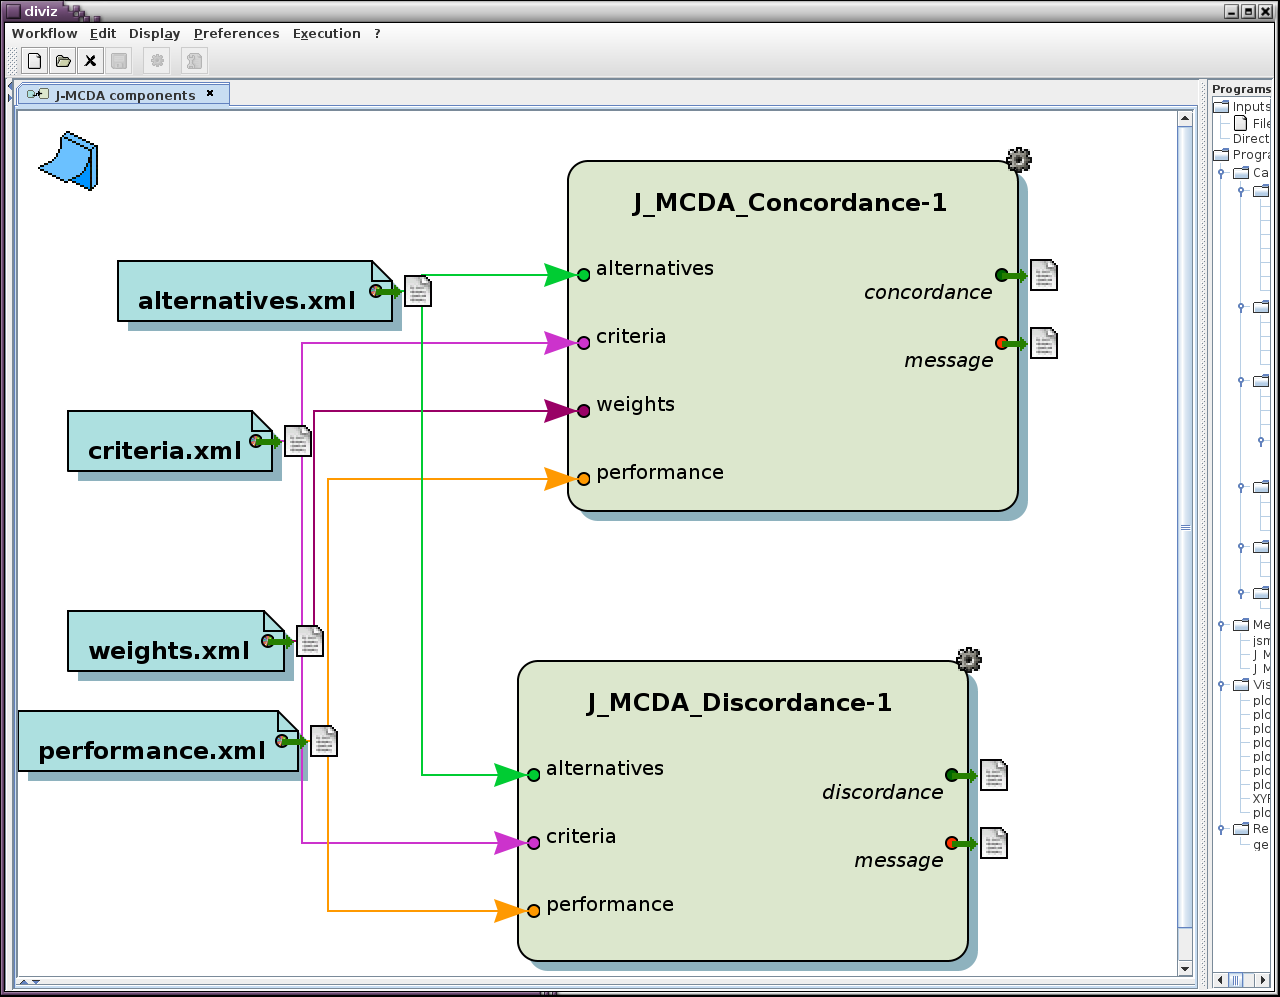
\includegraphics[width=\columnwidth, height=3.5cm, keepaspectratio]{diviz-J-MCDA-components.png}
\end{frame}

\section{À vous}
\begin{frame}
	\frametitle{À faire}
	\begin{itemize}
		\item Lisez (ou redirigez) vos e-mails @ Dauphine (pour les annonces)
		\item Installer les outils sur votre machine : Eclipse Mars Java EE, Java EE 7 (et Glassfish 4), Java 8 (OpenJDK)
		\item Choix d’un projet sur \href{https://mycourse.dauphine.fr/webapps/blackboard/execute/courseMain?course_id=_34753_1}{MyCourse}
		\item Présentation (5 à 10 min) de vos idées
		\item Compte \href{https://github.com/}{GitHub} ou \href{https://bitbucket.org/}{Bitbucket} et commit initial : diapos
	\end{itemize}
\end{frame}

\begin{frame}
	\frametitle{Sondage !}
	\begin{itemize}
		\item Avez-vous une machine à amener en cours ?
		\item Y a-t-il des prérequis qui vont vous manquer ?
		\item Sur quoi le cours devrait-il porter ?
	\end{itemize}
\end{frame}

\appendix
\AtBeginSection{
}
\section{Licence}
\begin{frame}
	\frametitle{Licence}
	Cette présentation, et le code LaTeX associé, sont sous \href{http://opensource.org/licenses/MIT}{licence MIT}. Vous êtes libres de réutiliser des éléments de cette présentation, sous réserve de citer l’auteur.
	
	Le travail réutilisé est à attribuer à \href{http://www.lamsade.dauphine.fr/~ocailloux/}{Olivier Cailloux}, Université Paris-Dauphine.
	
	\small{(Ceci ne couvre pas les images incluses dans ce document, puisque je n’en suis généralement pas l’auteur.)}
\end{frame}
\end{document}

